\documentclass[12pt]{article}
\usepackage[margin=0.5in]{geometry}



\usepackage{graphicx}
%\usepackage{amsmath}
%\usepackage{amsfonts}
%\usepackage{amssymb}
%\usepackage{amsthm}
%\usepackage{multicol}
%\usepackage{algorithms}
%\usepackage{showkeys}

%\newtheorem{Definition}{Definition}
%\newtheorem{Lemma}{Lemma}
%\newtheorem{Corollary}{Corollary}
%\newtheorem{Proposition}{Proposition}
%\newtheorem{Theorem}{Theorem}
%\newtheorem{Conjecture}{Conjecture}
%\newtheorem{Remark}{Remark}
%\newtheorem{question}{Question}
%\newtheorem{QaA}[question]{Q\&A}


\begin{document}

\title{Angry Ants: Midsemester Report}
%\date{\today}
\author{Paul Mueller and Jasmin Uribe}
\maketitle
\abstract Analyzing the motion and behavior of social insects requires tracking many individuals over time. Automated tracking is unreliable and inefficient. Ants frequently interact with each other which can cause the algorithm to begin tracking a different ant. The high density of ants being observed also increases the complexity of automated tracking. The authors of \cite{Joy12} use a ``citizen scientist" model where volunteers track ants then a representative trajectory is extracted for each ant using Frechet average and median trajectory. The authors also propose a global approach in which all ant trajectories are considered simultaneously. In this paper we construct this trajectory graph, $G$, and explore several methods of extracting a representative trajectory for each ant. We also propose an alternative method of determining trajectories based on DNA shot-gun sequencing. At the moment, we present the graph creating algorithm as well as provide a preliminary statisitical analysis of the data.

\section{Introduction}
\indent Biologists are exploring the social dynamics of ant colonies in order to better understand social organization in animal groups. In studying ant colonies, data is collected by tracking ant motion and interactions. Following each individual ant manually is impractical and time consuming. Automated tracking algorithms are unreliable and inefficient. Ants interact frequently by meeting, touching or crawling over each other. This makes tracking an individual ant difficult for an automated system. 
\indent The authors of \cite{Joy12} have created a prototype system that allows volunteers to track ants in videos in order to apply the ``citizen-scientist" model to this problem. The system extracts average trajectories using a ``local" approach: a representative trajectory for ant $x$ is computed using either a Frechet average or median trajectory. The authors then compared these representative trajectories to an existing automated ant tracking system and to the `ground truth'. See Fig. \ref{fig:ALocal}.

\begin{figure}
\centering
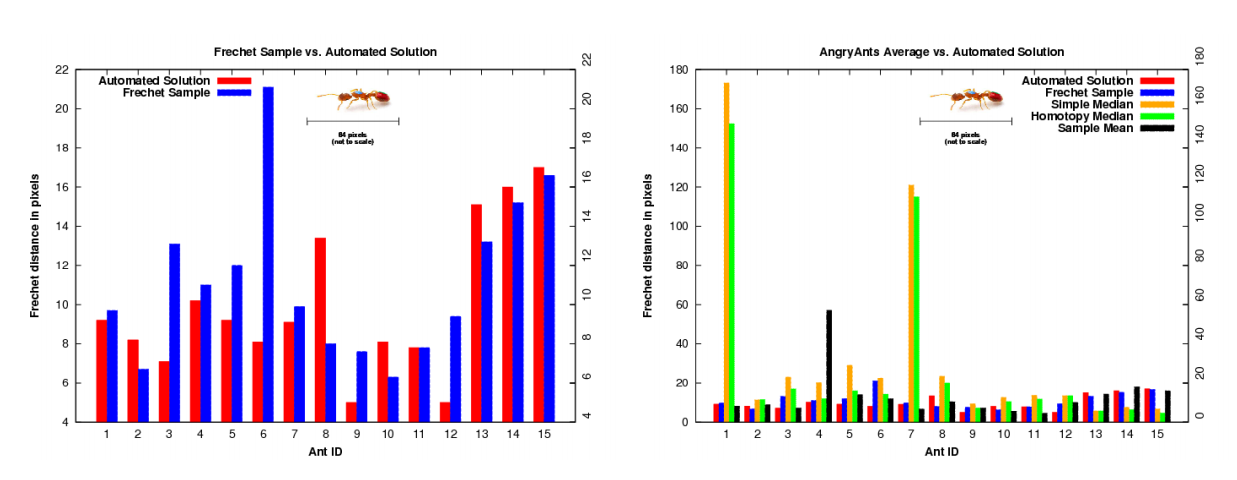
\includegraphics[width = 6.2in]{AntsJU.png}
\caption{Frechet distance between trajectories and `ground truth' \cite{Joy12}}
\label{fig:ALocal}
\end{figure}

\indent A complementary ``global" approach is described briefly in \cite{Joy12}. In this approach they consider trajectories for all $k$ ants together and construct a graph $G$ from these paths. The edges represent partial ant trajectories and the vertices are starting points, ending points or crossing points. See Fig. \ref{fig:AGraph}. Points where two or more ants meet are where citizen scientists mistakenly switch from tracking one ant to tracking another. The global approach is motivated by this phenomenon; trajectories of other ants may contain valid pieces of the path for ant $x$. \\

\begin{figure}[h!]
\centering
\includegraphics[width = 3.7in]{Antgraph.png}
\caption{Trajectory graph $G$ \cite{Joy12}}
\label{fig:AGraph}
\end{figure}

\indent In the unweighted case, the $x$-weight is proportional to the number of users who believe that ant $x$ moved through that edge between time $t_i$ and $t_{i+1}$. In order to find the $k$ edge-disjoint paths that begin at the source, end at the sink and cover all edges of $G$, a network flow instance is created. The difficulty here is the solution of the network flow may choose an inappropriate sequence of edges as the trajectory for a given ant. Thus the goal becomes compute a network flow with $k$ paths of different colors with the extra constraints so that each path is `feasible' and `optimal'. These extra constraints mean that the problem is neither the standard network flow problem nor a multi-commodity flow problem.


\indent Although some theoretical work has been done on the global approach, a trajectory graph, $G$, created with actual data has not been tested. Using the data collected for the local approach analysis in \cite{Joy12}, we create the trajectory graph and explore the representative trajectories extracted by several algorithms. We then compare the resulting trajectories to the `ground truth'. Finally we propose a new algorithm to extract ant trajectories based on DNA shot-gun sequencing.

\indent This paper is organized as follows. Related work is described in Section 2. Section 3 contains the graph generating algorithms. Section 4 details the proposed Shot-gun method as well a preliminary statistical analysis. Section 5 provides results and conclusions.

\section{Related Work}
Object tracking is defined as the problem of estimating the trajectories of certain objects in an image as they move around a defined space. Other relevant data such as orientation, shape and area of an object may be collected as well. Tracking objects is complex in many ways due to noise in the images, complex object motion, illumination changes and loss of the third dimension in 2D images, to name a few. Many approaches have been proposed for this problem, each addressing a slightly different issue.\\
\indent  \cite{Yilmaz06}  by Yilmaz {\it et al.} provides a survey of tracking methods grouped into broad categories. The purpose of the paper is to provide a library of tracking algorithms allowing readers to select the most appropriate based on their needs. They discuss the importance of object representation, object appearance, feature selection, object detection, background subtraction, and image segmentation. Different types of object tracking- point tracking, kernel tracking and silhouette tracking- are also discussed, as well as which algorithms are best suited to each. \\
\indent The authors of \cite{Maitra09} present a method for tracking bees that uses static and adaptive appearance templates as well as ``geometry-constrained resampling of particles for handling appearance change." Tracking bees, much like tracking ants, is difficult since the objects are all very similar and the appearance of an object can change over time. With bees, the placement of the wings, the orientation of the bee, and the uneven lighting affect how the bee will appear in the image. Appearance templates provide a more complete description of the appearance, making the algorithm more sensitive to specific features of the bee. The added resampling step improves the prediction of head and thorax orientation. Together these modifications improve tracking when compared to a particle filtering based tracking with Gaussian modeling of appearance.\\
\indent In a more recent paper, \cite{Fletcher11} present a method for tracking multiple ants. They ``prevent drifts by maximizing the coverage of foreground pixels at a global scale" and ``improve speed by reducing Markov chain length through dynamically changing the target proposal distribution for perturbed ant selection." They used the fact that in many cases the number of ants being tracked remained constant for a certain period of time combined with the assumption that all ant pixels are tracked to reduce the algorithm erroneously switching from one ant path to another. They also increased efficiency by using a ``variable target proposal distribution." Not all ants move at every time step, so instead of using a fixed distribution they dynamically vary the distribution based on the level of expected motion. These changes improve both accuracy and speed.\\
\indent One of the major problems with automatic tracking methods is drifting, which occurs when the tracker loses the object it is tracking. In 2012, \cite{Poff12} addressed this problem by enabling a user to examine a fraction of the entire sequence for validating and correcting mis-trackings. Frames containing drifts were identified ``based on the amount of un-tracked foreground pixels;" this modification improved automated tracking by 25\%.\\
\indent Markov chain Monte Carlo based particle filters were used by \cite{Zuria08} to effectively deal with interacting targets whose behavior is dependent on its interactions with others. They propose a model that maintains the identity of the objects throughout an interaction in order to reduce drifting. The algorithm is based on the assumption that certain objects do not behave independently, but rather an encounter between two objects can result in very different behavior. This paper demonstrates how ``a Markov random field motion prior, built on the fly at each time step, can adequately model these interactions."\\
\indent Once the data has been collected, using an automated tracking algorithm or otherwise, it must then be analyzed. There are two general approaches: the local approach, in which we consider individual trajectories, and the global approach, in which we consider all trajectories. Some research has been done on determining an average path given a data set of many paths and much work has been done on averaging polygonal paths. In \cite{Morris}, they present an approach for finding recreational trails using aerial images and maps. They assume the two end points of the trail are given, then find the most likely trail between the points. They estimate the likelihood that an observed piece of an image is on the trail using three different models. They then integrate this approach with a more global approach by noting that pieces of a trail must link up to connect the start point with the end point. \\
\indent The authors of \cite{Buchin10} ``establish criteria that a `median trajectory' should meet" then present methods of computing said median. Two of the properties of a median trajectory are that any point, $p$, on the median must also lie on an input trajectory and the minimum number of distinct trajectories $p$ must cross to reach the unbounded face is $\frac{m+1}{2}$, where $m$ is the number of input trajectories. The authors of \cite{Joy12} use this definition of a median trajectory in one of the local approaches.\\
\indent When considering the local approach, it is necessary to define a measure of how close one path is to another. In many papers the Frechet distance is used. In \cite{Driemel10} a practical approximation algorithm is presented for the Frechet distance between two polygonal curves. The Frechet distance can be thought of as the maximum distance a point on the first curve has to travel as this curve is being continuously deformed into the second curve. A new class of curves for which the Frechet distance can be approximated quickly is introduced.\\
\indent The authors of `Matching Planar Maps' by {\it Alt et al.} \cite{Alt03} present an algorithm ``for measuring the similarity patterns of line segments in the plane." They consider a polygonal curve and an embedded graph with line segment edges. The goal is to find a path in the graph that minimizes the Frechet distance between the path and the curve. This idea is modified in \cite{Buchin09} where exact algorithms are determined for partial curve matching using Frechet distance. Here, they measured partial similarity between curves. The goal was to maximize the total length of subcurves that are close to each other. They present a polynomial-time exact algorithm for computing this maximum.\\
\indent \cite{Blum2008ant} presents a version of sequencing by hybridization using an ant colony optimization algorithm. Applies the basic ACO algorithm within a "multilevel framework", which reduces a problem to smaller instances by successive coarsening until a stopping criteria is reached. This paper also includes a list of papers detailing other approaches to SBH.\\
\indent \cite{Li2008map} describes a DNA sequence mapping algorithm that is well suited to efficiently aligning large amounts of short reads (30 - 40 base pairs) to a reference genome. Also described is a method to determine the confidence that such mapping was performed correctly. The source code is freely available.\\
\indent As mentioned, the authors of \cite{Joy12} have done some analysis on the local approach using Frechet average and median trajectories. There is also work being done using a $k$-clustering algorithm, in which ant movement is visualized in 3D with time as the $z$-axis (unpublished Yunhao). Each frame is a horizontal slice through the $z$-axis. Each ant is a point and ants intersect when points are clustered sufficiently close together. \\
\indent Currently there is experimental work being done on a linear programming approach to solve the global network flow problem (unpublished Alon/Sergei). In this case, weights are assigned to each edge for each ant. These weights should add up to 1. The goal is to maximize the $(weight)*(cost)$ over all edges and all ants.  For each vertex, the sum of incoming weights of each ant should equal the sum of outgoing weights of that particular ant. The conjuncture is that for each edge the weight of one ant will be 1 and the weight of all other ants will be 0. It is simple to prove this for two ants; however, it is not clear how this generalizes to more than two ants. Experimentally, this conjecture has been shown for three ants. Most recently a proof has been proposed demonstrating the solution will be integer in the most general case. \\



\section{Creating the Trajectory Graph}
In order to test the accuracy of the global approach we must first create a trajectory graph, $G$. We do this in two ways. The first uses simulated data, ie. simulated ant trajectories, and the second is based on user-collected trajectories. We use the same data set used in \cite{Joy12}. They used a video with about 10,000 frames recorded at 30 frames per second of a {\it Temnothorax rugatulus} ant colony. 
\subsection{Random Graph Generator}

This is a Python program that generates a graph consisting of disconnected
components representing tracings of a given number of ants, where the tracings
are contributed by simulated users.\\
\indent It first creates the ant trails, with the ants moving around randomly: they tend
to keep going in the direction they are already moving in, but can change
direction at each time step such that the larger the change, the less likely it
is to occur, following a bell-curve probability.\\
\indent After the actual trails are generated, a requested number of "users" track each
ant, with their "clicks" being within a requested distance of the ant's actual
position in the current time step. However, they can also become confused, and
start tracking a different ant if it is close enough.\\
\indent This program allows us to generate as much test data as needed and validate our
algorithms' performance on it, as the generator provides both the simulated
ground-truth ant-trail data and the tracking data of the simulated users. Since
the program is configurable, we are able to generate data with various
properties, allowing us to test our algorithms more effectively. We will use
this in conjunction with the real-world data.


\subsection{Crossings Graph Creator}

This is a Python program that converts our real-world data into a graph, and
from there into LEMON \cite{LEMON} text graph format if requested.\\
\indent It takes as input a set of data points representing the position a user observed during the current time step, for all user data. There are multiple users tracking each ant throughout the duration of the experiment.\\
\indent It then creates a graph of the user data that has a vertex at each ant position
at each time step, and an edge from each vertex in a given time step to each
vertex in the next time step. The edges each have a weight for each ant in the
experiment; the weight for ant $a$ gives the number of users $n$ who thought
that ant traveled along that path.\\
\indent The graph creation uses the hierarchical/agglomerative clustering algorithm
of Scipy \cite{Scipy} to perform the clustering at each time step, without
specifying a-priori how many clusters there are. This is necessary because the
number of clusters at a given time step will vary, as ants move closer and
farther away from each other.



\subsection{Min-Cost Flow, One-Ant-At-A-Time Global Weighted Algorithm}

This is an in-progress implementation of the algorithm mentioned in section 2.2
of the AngryAnts paper. It is implemented in C++ using the network simplex
algorithm of the LEMON graph library \cite{LEMON}.\\
\indent This algorithm considers the path each ant took from its starting vertex at the
first time step to a vertex in the last time step as a separate min-cost flow
problem. After computing the flow for a given ant, it removes all the edges used
by that ant from consideration for future ant paths. This ensures that all the
user-contributed edges are used, but may not find the optimal paths for all
ants, as an earlier min-cost-flow application may use edge(s) that would have
been better used by a later application.\\
\indent For each ant being tracked, the algorithm sets the cost of each edge in the
graph to the total number of users minus the number of users who thought that
ant used the edge in question. The edge capacities are not used (each is set to
infinity), as the costs by themselves are sufficient. The source and sink
capacities are set to 1 and -1, respectively, to ensure that each ant follows a
single path (i.e., it does not split up into multiple "sub-ants", which
clearly makes no sense).\\
\indent This program makes use of LEMON's built-in text graph data file format to accept
its input. The graph generator is capable of generating output in this format,
and the crossings graph creator mentioned above converts our real-world data
into LEMON text graph format.


% The goal of this project is to create an algorithm that computes a network flow as described above such that each path is `feasible' and `optimal'.  We will begin by exploring a simple Greedy algorithm then the min-cost flow problem and, as suggested by \cite{Joy12}, implement an algorithm that finds the optimal path for ant $A$ and removes these paths, then ant $B$, removes these paths, etc. \\
%
%
%
%\begin{center}\begin{tabular}{|c|c|c|c|c|}
%	\hline Algorithm & local/global & time & implemented?& Who? \\
%	\hline Frechet & local & No & Yes & \cite{Joy12} \\
%	\hline Median & local & No & Yes & \cite{Joy12} \\
%	\hline MC Basic & global & Yes & pilot test & Paul, Jasmin \\
%	\hline Lin. Prog. & global & Yes & up to 3 & Sergei\\
%	\hline k-Clustering & global & Yes & in prog & Yunhao\\
%	\hline Shotgun & global & Yes & No & Paul, Jasmin\\
%	\hline
%	\end{tabular}\end{center}
%
%
%\indent In order to determine how far the paths we generate are from the `ground truth' we will use least squares distance and Frechet distance. If needed, we may develop a new metric specific to the data in order to evaluate the distance between paths.\\
%\indent If time permits we will explore the effectiveness and efficiency of various validation schemes.

\section{Shotgun Method}
\indent We propose an alternative approach based on shotgun sequencing in DNA \cite{Anson10}. We notice that over time users tend to lose interest in tracing the ant path. This results in more errors in the data as time increases. We take advantage of the initial, more accurate portions of the path by initializing path-tracing at different times. For example, suppose we wish to track ant $A$. We ask $n$ users to track ant $A$, where each user begins tracking at a different time $\{t_1,...,t_n\}$. Taking these $n$ paths we will then identify the portions that are at the same time step. We can then `glue' the paths together at these matching portions and ultimately, determine a resulting path that is a continuous curve from start time to end time.\\
\indent In the implementation of this approach there are three factors to test: the partition of initial observation times, the distribution of observation lengths, and the maximum observation time before the observer begins to lose interest. In the initial implementation, the starting times will be equally spaced- in other words, the partition will be uniform. We can begin by requiring that all observers trace the path for a fixed amount of time. \\
\subsection{Algorithm}
This method is based on DNA shot-gun sequencing, a method used to sequence large amounts of genetic material, the entire human genome, for example. The premise of the method is that a long fragment of genetic code can be sequenced by sequencing shorter randomly selected segments that overlap then `glueing' these segments together at the overlaping regions. This method decreases the error since mistakes are less likely to occur when sequencing shorter segments. Similarly, when tracking ants, the user is more likely to lose interest and make a mistake the longer they trace a trajectory. Taking this into consideration, we propose the shot-gun method for determining ant trajectories. \\
\indent We begin by describing the data collection phase of the method. Previoulsy, users were asked to track a specific ant for exactly the same fragment of video. In this method, each observation will be initialized at a random time and ultimately the length of each fragment will also be randomly distributed. A new segment will be chosen until every time has been tracked at least 5 times. These segments will then be pieced together according to the time stamp. There will be five different data points associated to each time step. If all are within 17 pixels, an average will be taken and this will be a point on the representative trajectory. If there is an outlier, we determine if this was at the start of a trace or the end of a trace and weight this value appropriately or we use the trajectory graph to determine if an error occured at a crossing. 
\subsection{Preliminary Statistical Analysis}
We run the preliminary analysis on the same data set used in \cite{Joy12}. They used a video with about 10,000 frames recorded at 30 frames per second of a {\it Temnothorax rugatulus} ant colony. 
Given the number of ants in the frame and the `ground truth' trajectory for each ant we beign by selecting an ant at random using a uniformly distributed discrete random variable. We then select a random time/place pair from the `ground truth' data for this ant. The game will be initialized at this time and place. We begin by having users track for a fixed amount of time then we run a second round of experiments where users track for a randomly distributed amount of time. \\
\indent We must ensure that each point in the trajectory is traced sufficiently many times in order to minimize the error. We calculate this number using the orginal data set used in the local trajecotry analysis. We use the standard deviation of  the distance from each observed point to the ground truth.
%Let $X_{i}^{a}$ be the `ground truth' position of ant $a$ at time $i$. Let $\{Y_{1,i}, ...Y_{n,i}\}$ be the position of ant $a$ at time $i$ as observed by $n$ users. We determine the standard deviation $ S = \sqrt{\frac{1}{n}\sum\limits_{j =1}^n {(Y_{j,i}-X_i^a)^2}}$.
 For example, for Ant5 six users collected data. We look at the following frames \{1,101,201,301...,3301\}. For each user and each frame we compute the square of the Euclidean distance from the observed point to the ground truth. We then compute the average square distance across all users for each time frame. The square root of this number is the standard deviation. Since an ant is assumed to be 17 pixels long, we took a ball of radius $\frac{17}{2}$ as a threshold. If the standard deviation falls within this ball, we assume the observations to be exact. \\
\indent We perform this analysis for Ant5, Ant6, Ant27, Ant36, and Ant44. For Ants 5,6,27, and 36, the standard deviation fell beneath the threshold for almost every time frame, in the few cases it did not, the deviation was less than 2 pixels. These results demonstrate that the observations are reliable and that we do not need to introduce any considerations to reduce observational error. Ant44 was tracked by 8 users. After time frame 101, however, one user's standard deviation increased significantly. When cross-refernecing the orginal data file it was clear this user was now tracking a stationary ant, whose path did not match any of the other 7 users. Once this outlying path was eliminated from the data, the standard deviation dropped below the threshold. \\
\indent This interesting event with Ant44 highlights several aspects of this statistical analysis. First, given that the standard deviation of the observed paths is quite low, it easy to determine when a user begins tracking another ant and which user begins to do so. This means it is easy to identify and eliminate this path from the data set for the specific ant. In addition, if we have a complete trajectory graph, we can cross reference this graph in order to determine which ant the outlying path could belong to. For example, for Ant44 we know one user began to deviate after frame 101, using this we can reference the graph and determine which ant crossed paths with Ant44 between frames 101 and 201, then see if the deviant path matches the path of this other ant. If so, we can add this path to the data set for this ant instead. Thus eliminating this path from one data set while using it in another more appropriate data set. If this method is used, It is important that dat is collected for every ant in the frame and the trajectory graph is compete, otherwise, it is not possible to detemine if the deviant path belongs to another ant. \\
\section{Results, Conclusions, and Future Work}
Results from the preliminary statistical analysis demonstrate that a basic standard deviation analysis can pinpoint when and which users began tracking a different ant. This, in conjunction with the trajectory graph data, can aid in removing that path from the data of the original ant and adding it to the data set of another. This allows all data, even seemingly `incorrect' data, to be used. \\
\indent We are currently in the process of gathering data in order to test the shot-gun method. Once the user data has been gathered, the accuracy and efficiency of the shot-gun method can be assessed. We will test the shot-gun method using simulated data in order to refine the algorithm and remedy any unforseen issues.


\newpage
\bibliography{hayley}
\bibliographystyle{plain}

\end{document}
